% Options for packages loaded elsewhere
% Options for packages loaded elsewhere
\PassOptionsToPackage{unicode}{hyperref}
\PassOptionsToPackage{hyphens}{url}
\PassOptionsToPackage{dvipsnames,svgnames,x11names}{xcolor}
%
\documentclass[
  12pt,
  oneside,
  a4paper,
  english,
  brazil]{abntex2}
\usepackage{xcolor}
\usepackage[top=30mm,left=30mm,right=20mm,bottom=20mm]{geometry}
\usepackage{amsmath,amssymb}
\setcounter{secnumdepth}{5}
\usepackage{iftex}
\ifPDFTeX
  \usepackage[T1]{fontenc}
  \usepackage[utf8]{inputenc}
  \usepackage{textcomp} % provide euro and other symbols
\else % if luatex or xetex
  \usepackage{unicode-math} % this also loads fontspec
  \defaultfontfeatures{Scale=MatchLowercase}
  \defaultfontfeatures[\rmfamily]{Ligatures=TeX,Scale=1}
\fi
\usepackage{lmodern}
\ifPDFTeX\else
  % xetex/luatex font selection
\fi
% Use upquote if available, for straight quotes in verbatim environments
\IfFileExists{upquote.sty}{\usepackage{upquote}}{}
\IfFileExists{microtype.sty}{% use microtype if available
  \usepackage[]{microtype}
  \UseMicrotypeSet[protrusion]{basicmath} % disable protrusion for tt fonts
}{}
\makeatletter
\@ifundefined{KOMAClassName}{% if non-KOMA class
  \IfFileExists{parskip.sty}{%
    \usepackage{parskip}
  }{% else
    \setlength{\parindent}{0pt}
    \setlength{\parskip}{6pt plus 2pt minus 1pt}}
}{% if KOMA class
  \KOMAoptions{parskip=half}}
\makeatother
% Make \paragraph and \subparagraph free-standing
\makeatletter
\ifx\paragraph\undefined\else
  \let\oldparagraph\paragraph
  \renewcommand{\paragraph}{
    \@ifstar
      \xxxParagraphStar
      \xxxParagraphNoStar
  }
  \newcommand{\xxxParagraphStar}[1]{\oldparagraph*{#1}\mbox{}}
  \newcommand{\xxxParagraphNoStar}[1]{\oldparagraph{#1}\mbox{}}
\fi
\ifx\subparagraph\undefined\else
  \let\oldsubparagraph\subparagraph
  \renewcommand{\subparagraph}{
    \@ifstar
      \xxxSubParagraphStar
      \xxxSubParagraphNoStar
  }
  \newcommand{\xxxSubParagraphStar}[1]{\oldsubparagraph*{#1}\mbox{}}
  \newcommand{\xxxSubParagraphNoStar}[1]{\oldsubparagraph{#1}\mbox{}}
\fi
\makeatother

\usepackage{color}
\usepackage{fancyvrb}
\newcommand{\VerbBar}{|}
\newcommand{\VERB}{\Verb[commandchars=\\\{\}]}
\DefineVerbatimEnvironment{Highlighting}{Verbatim}{commandchars=\\\{\}}
% Add ',fontsize=\small' for more characters per line
\newenvironment{Shaded}{}{}
\newcommand{\AlertTok}[1]{\textcolor[rgb]{1.00,0.33,0.33}{\textbf{#1}}}
\newcommand{\AnnotationTok}[1]{\textcolor[rgb]{0.42,0.45,0.49}{#1}}
\newcommand{\AttributeTok}[1]{\textcolor[rgb]{0.84,0.23,0.29}{#1}}
\newcommand{\BaseNTok}[1]{\textcolor[rgb]{0.00,0.36,0.77}{#1}}
\newcommand{\BuiltInTok}[1]{\textcolor[rgb]{0.84,0.23,0.29}{#1}}
\newcommand{\CharTok}[1]{\textcolor[rgb]{0.01,0.18,0.38}{#1}}
\newcommand{\CommentTok}[1]{\textcolor[rgb]{0.42,0.45,0.49}{#1}}
\newcommand{\CommentVarTok}[1]{\textcolor[rgb]{0.42,0.45,0.49}{#1}}
\newcommand{\ConstantTok}[1]{\textcolor[rgb]{0.00,0.36,0.77}{#1}}
\newcommand{\ControlFlowTok}[1]{\textcolor[rgb]{0.84,0.23,0.29}{#1}}
\newcommand{\DataTypeTok}[1]{\textcolor[rgb]{0.84,0.23,0.29}{#1}}
\newcommand{\DecValTok}[1]{\textcolor[rgb]{0.00,0.36,0.77}{#1}}
\newcommand{\DocumentationTok}[1]{\textcolor[rgb]{0.42,0.45,0.49}{#1}}
\newcommand{\ErrorTok}[1]{\textcolor[rgb]{1.00,0.33,0.33}{\underline{#1}}}
\newcommand{\ExtensionTok}[1]{\textcolor[rgb]{0.84,0.23,0.29}{\textbf{#1}}}
\newcommand{\FloatTok}[1]{\textcolor[rgb]{0.00,0.36,0.77}{#1}}
\newcommand{\FunctionTok}[1]{\textcolor[rgb]{0.44,0.26,0.76}{#1}}
\newcommand{\ImportTok}[1]{\textcolor[rgb]{0.01,0.18,0.38}{#1}}
\newcommand{\InformationTok}[1]{\textcolor[rgb]{0.42,0.45,0.49}{#1}}
\newcommand{\KeywordTok}[1]{\textcolor[rgb]{0.84,0.23,0.29}{#1}}
\newcommand{\NormalTok}[1]{\textcolor[rgb]{0.14,0.16,0.18}{#1}}
\newcommand{\OperatorTok}[1]{\textcolor[rgb]{0.14,0.16,0.18}{#1}}
\newcommand{\OtherTok}[1]{\textcolor[rgb]{0.44,0.26,0.76}{#1}}
\newcommand{\PreprocessorTok}[1]{\textcolor[rgb]{0.84,0.23,0.29}{#1}}
\newcommand{\RegionMarkerTok}[1]{\textcolor[rgb]{0.42,0.45,0.49}{#1}}
\newcommand{\SpecialCharTok}[1]{\textcolor[rgb]{0.00,0.36,0.77}{#1}}
\newcommand{\SpecialStringTok}[1]{\textcolor[rgb]{0.01,0.18,0.38}{#1}}
\newcommand{\StringTok}[1]{\textcolor[rgb]{0.01,0.18,0.38}{#1}}
\newcommand{\VariableTok}[1]{\textcolor[rgb]{0.89,0.38,0.04}{#1}}
\newcommand{\VerbatimStringTok}[1]{\textcolor[rgb]{0.01,0.18,0.38}{#1}}
\newcommand{\WarningTok}[1]{\textcolor[rgb]{1.00,0.33,0.33}{#1}}

\usepackage{longtable,booktabs,array}
\usepackage{calc} % for calculating minipage widths
% Correct order of tables after \paragraph or \subparagraph
\usepackage{etoolbox}
\makeatletter
\patchcmd\longtable{\par}{\if@noskipsec\mbox{}\fi\par}{}{}
\makeatother
% Allow footnotes in longtable head/foot
\IfFileExists{footnotehyper.sty}{\usepackage{footnotehyper}}{\usepackage{footnote}}
\makesavenoteenv{longtable}
\usepackage{graphicx}
\makeatletter
\newsavebox\pandoc@box
\newcommand*\pandocbounded[1]{% scales image to fit in text height/width
  \sbox\pandoc@box{#1}%
  \Gscale@div\@tempa{\textheight}{\dimexpr\ht\pandoc@box+\dp\pandoc@box\relax}%
  \Gscale@div\@tempb{\linewidth}{\wd\pandoc@box}%
  \ifdim\@tempb\p@<\@tempa\p@\let\@tempa\@tempb\fi% select the smaller of both
  \ifdim\@tempa\p@<\p@\scalebox{\@tempa}{\usebox\pandoc@box}%
  \else\usebox{\pandoc@box}%
  \fi%
}
% Set default figure placement to htbp
\def\fps@figure{htbp}
\makeatother


% definitions for citeproc citations
\NewDocumentCommand\citeproctext{}{}
\NewDocumentCommand\citeproc{mm}{%
  \begingroup\def\citeproctext{#2}\cite{#1}\endgroup}
\makeatletter
 % allow citations to break across lines
 \let\@cite@ofmt\@firstofone
 % avoid brackets around text for \cite:
 \def\@biblabel#1{}
 \def\@cite#1#2{{#1\if@tempswa , #2\fi}}
\makeatother
\newlength{\cslhangindent}
\setlength{\cslhangindent}{1.5em}
\newlength{\csllabelwidth}
\setlength{\csllabelwidth}{3em}
\newenvironment{CSLReferences}[2] % #1 hanging-indent, #2 entry-spacing
 {\begin{list}{}{%
  \setlength{\itemindent}{0pt}
  \setlength{\leftmargin}{0pt}
  \setlength{\parsep}{0pt}
  % turn on hanging indent if param 1 is 1
  \ifodd #1
   \setlength{\leftmargin}{\cslhangindent}
   \setlength{\itemindent}{-1\cslhangindent}
  \fi
  % set entry spacing
  \setlength{\itemsep}{#2\baselineskip}}}
 {\end{list}}
\usepackage{calc}
\newcommand{\CSLBlock}[1]{\hfill\break\parbox[t]{\linewidth}{\strut\ignorespaces#1\strut}}
\newcommand{\CSLLeftMargin}[1]{\parbox[t]{\csllabelwidth}{\strut#1\strut}}
\newcommand{\CSLRightInline}[1]{\parbox[t]{\linewidth - \csllabelwidth}{\strut#1\strut}}
\newcommand{\CSLIndent}[1]{\hspace{\cslhangindent}#1}



\setlength{\emergencystretch}{3em} % prevent overfull lines

\providecommand{\tightlist}{%
  \setlength{\itemsep}{0pt}\setlength{\parskip}{0pt}}



 


% ---
% Pacotes básicos 
% ---
\usepackage{lmodern}			% Usa a fonte Latin Modern			
\usepackage[T1]{fontenc}		% Selecao de codigos de fonte.
\usepackage[utf8]{inputenc}		% Codificacao do documento (conversão automática dos acentos)
\usepackage{lastpage}			% Usado pela Ficha catalográfica
\usepackage{indentfirst}		% Indenta o primeiro parágrafo de cada seção.
\usepackage{color}				% Controle das cores
\usepackage{graphicx}			% Inclusão de gráficos
\usepackage{microtype} 			% para melhorias de justificação
\usepackage{listings}			% Inclusão de código fonte 			


% Pacotes de citações
% ---
\usepackage[brazilian,hyperpageref]{backref}	 % Paginas com as citações na bibl
\usepackage[alf]{abntex2cite}	% Citações padrão ABNT

% --- 
% CONFIGURAÇÕES DE PACOTES
% --- 

% ---
% Configurações do pacote backref
% Usado sem a opção hyperpageref de backref
\renewcommand{\backrefpagesname}{Citado na(s) página(s):~}
% Texto padrão antes do número das páginas
\renewcommand{\backref}{}
% Define os textos da citação
\renewcommand*{\backrefalt}[4]{
	\ifcase #1 %
		Nenhuma citação no texto.%
	\or
		Citado na página #2.%
	\else
		Citado #1 vezes nas páginas #2.%
	\fi}%
% ---

% ---
% Configurações de aparência do PDF final

% alterando o aspecto da cor azul
\definecolor{blue}{RGB}{41,5,195}
% informações do PDF
\makeatletter

\hypersetup{
     	%pagebackref=true,
		% pdftitle={\@title}, 
		% pdfauthor={\@author},
    	% pdfsubject={\imprimirpreambulo},
	    % pdfcreator={LaTeX with abnTeX2},
		% pdfkeywords={abnt}{latex}{abntex}{abntex2}{trabalho acadêmico}, 
		colorlinks=true,       		% false: boxed links; true: colored links
    	linkcolor=blue,          	% color of internal links
    	citecolor=blue,        		% color of links to bibliography
    	filecolor=magenta,      		% color of file links
		urlcolor=blue,
		bookmarksdepth=4
}

% Comandos de uso do orientador para sugestão de alterações:
\usepackage{xcolor}
\usepackage{cancel}

\colorlet{oliveGreen}{blue!20!black!50!green}

\usepackage{soul}
\usepackage{soulutf8}
\setstcolor{red}

\newcommand{\cito}[1]{\textsuperscript{\cite{#1}}} % numeração da citação sobreescrita
\newcommand{\PROFESSOR}[1]{\textcolor{red}{\MakeUppercase{#1}}} % Acrescenta um nota pelo professor
\newcommand{\PROFESSORDEL}[1]{\textcolor{red}{\st{#1}}} % removido pelo professor
\newcommand{\PROFESSORADD}[1]{\textcolor{oliveGreen}{#1}} % adicionado pelo professor
\newcommand{\PROFESSORREP}[2]{\PROFESSORDEL{#1}\PROFESSORADD{#2}} % substituir


\renewcommand{\printtoctitle}[1]{\ABNTEXchapterfontsize\centering SUMÁRIO}

\AtBeginDocument{\captionsetup{labelfont=bf}}





\makeatother
% --- 

% --- 
% Espaçamentos entre linhas e parágrafos 
% --- 

% O tamanho do parágrafo é dado por:
\setlength{\parindent}{1.3cm}

% Controle do espaçamento entre um parágrafo e outro:
\setlength{\parskip}{0.2cm}  % tente também \onelineskip

% ---
% compila o indice
% ---
\makeindex
% ---
\makeatletter
\@ifpackageloaded{caption}{}{\usepackage{caption}}
\AtBeginDocument{%
\ifdefined\contentsname
  \renewcommand*\contentsname{Table of contents}
\else
  \newcommand\contentsname{Table of contents}
\fi
\ifdefined\listfigurename
  \renewcommand*\listfigurename{Lista de Figuras}
\else
  \newcommand\listfigurename{Lista de Figuras}
\fi
\ifdefined\listtablename
  \renewcommand*\listtablename{Lista de Tabelas}
\else
  \newcommand\listtablename{Lista de Tabelas}
\fi
\ifdefined\figurename
  \renewcommand*\figurename{Figura}
\else
  \newcommand\figurename{Figura}
\fi
\ifdefined\tablename
  \renewcommand*\tablename{Tabela}
\else
  \newcommand\tablename{Tabela}
\fi
}
\@ifpackageloaded{float}{}{\usepackage{float}}
\floatstyle{ruled}
\@ifundefined{c@chapter}{\newfloat{codelisting}{h}{lop}}{\newfloat{codelisting}{h}{lop}[chapter]}
\floatname{codelisting}{Código}
\newcommand*\listoflistings{\listof{codelisting}{Lista de Códigos}}
\makeatother
\makeatletter
\makeatother
\makeatletter
\@ifpackageloaded{caption}{}{\usepackage{caption}}
\@ifpackageloaded{subcaption}{}{\usepackage{subcaption}}
\makeatother
\makeatletter
\@ifpackageloaded{tcolorbox}{}{\usepackage[skins,breakable]{tcolorbox}}
\makeatother
\makeatletter
\@ifundefined{shadecolor}{\definecolor{shadecolor}{rgb}{.97, .97, .97}}{}
\makeatother
\makeatletter
\makeatother
\makeatletter
\ifdefined\Shaded\renewenvironment{Shaded}{\begin{tcolorbox}[frame hidden, boxrule=0pt, borderline west={3pt}{0pt}{shadecolor}, interior hidden, sharp corners, breakable, enhanced]}{\end{tcolorbox}}\fi
\makeatother
\usepackage{bookmark}
\IfFileExists{xurl.sty}{\usepackage{xurl}}{} % add URL line breaks if available
\urlstyle{same}
\hypersetup{
  colorlinks=true,
  linkcolor={blue},
  filecolor={Maroon},
  citecolor={Blue},
  urlcolor={Blue},
  pdfcreator={LaTeX via pandoc}}


\author{}
\date{}
\begin{document}


\setlength{\parindent}{0mm}
\ABNTEXchapterfont\normalsize

\ABNTEXchapterfont\normalsize

\begin{center}
\uppercase{ Instituto Tecnológico de Aeronáutica }

\uppercase{ Divisão de Ciências Fundamentais }

\uppercase{ Programa de Pós-Graduação XYZ }

\vfill

\uppercase{ Nome Pessoa }

\vfill

\uppercase{ Template para TCC: }

Uso do quarto.org

\vfill

\uppercase{ São José dos Campos }

2025

\end{center}

\newpage{}

\begin{center}
\uppercase{ Nome Pessoa }

\vspace{6cm}

\uppercase{ Template para TCC: }

Uso do quarto.org

\vspace{3cm}

\hfill\begin{minipage}{0.5\textwidth}
Dissertação de Mestrado apresentado na Divisão de Ciências Fundamentais do Instituto Tecnológico de Aeronáutica como requisito básico para a conclusão do Curso de Mestrado Profissional UVW.

\vspace{1cm}

Orientador (a): São Jorge

Coorientador (a): Santa Maria

\end{minipage}

\vfill

\uppercase{ São José dos Campos }

2025

\end{center}

\newpage{}

\textbf{Dados Internacionais de Catalogação-na-Publicação (CIP)}

\textbf{Divisão de Informação e Documentação}

\vspace{-3mm}

\begin{framed}

\begin{center}
\begin{minipage}[c]{13.5cm}

\footnotesize

\vspace{-5mm}

Pessoa, Nome

\hspace{0.5cm} Template para TCC: / Pessoa, Nome - São José dos Campos, 2025.

\hspace{0.5cm} \pageref{LastPage} f.

\vspace{5mm}

\hspace{0.5cm} Dissertação de Mestrado - Curso de Mestrado Profissional UVW, Área de Engenharias III - Instituto Tecnológico de Aeronáutica, 2025.

\vspace{5mm}

\hspace{0.5cm} Orientador: Prof. Dr. São Jorge.

\hspace{0.5cm}
    1. palavra 1.
    2. palavra 2.
    3. palavra 3.
    4. palavra 4.
    5. palavra 4.
    I. São Jorge.
    II. Instituto Tecnológico de Aeronáutica.
    III. Programa de Pós-Graduação XYZ.
    IV. Template para TCC:\\            

\hspace{9.75cm} CDU C02:141:005.7\\

\vspace{-8mm}

\normalsize

\end{minipage}
\end{center}

\end{framed}

\vfill

\textbf{REFERÊNCIA BIBLIOGRÁFICA}

\uppercase{ Pessoa}, Nome. Template para TCC:. 2025. \pageref{LastPage}
f.~Dissertação de Mestrado - Curso de Mestrado Profissional UVW, Área de
Engenharias III - Instituto Tecnológico de Aeronáutica, São José dos
Campos, 2025.

\vfill

\textbf{CESSÃO DE DIREITOS}

\textbf{NOME DO AUTOR:} Nome Pessoa\\
\textbf{TÍTULO DO TRABALHO:} Template para TCC:\\
\textbf{TIPO DO TRABALHO/ANO:} Dissertação de Mestrado / 2025.

É concedida ao\{à\} Instituto Tecnológico de Aeronáutica a permissão
para reproduzir cópias desta Dissertação de Mestrado para emprestar ou
vender cópias, exclusivamente para fins acadêmicos e científicos. O
autor reserva os demais direitos de publicação, e nenhuma parte desta
dissertação ou tese poderá ser reproduzida sem sua autorização.

\vspace{1cm}

\begin{center}\rule{0.5\linewidth}{0.5pt}\end{center}

Nome Pessoa

Endereço Eletrônico: nome.pessoa@nomes.com

São José dos Campos-SP

\newpage{}

\begin{center}

\uppercase{ Nome Pessoa }

\vfill

\begin{center}
  \uppercase{ Template para TCC: }
  Uso do quarto.org
\end{center}

\end{center}

\vfill

Composição de Banca Examinadora:

\begin{center}

% Tabela sem linhas visíveis
\begin{tabular}{>{\raggedright\arraybackslash}p{6cm} >{\raggedright\arraybackslash}p{4cm} >{\raggedright\arraybackslash}p{3cm} >{\raggedright\arraybackslash}p{1cm} >{\raggedright\arraybackslash}p{3cm}}
 Prof. Dr. Sidarta Gautama    & Presidente     & - & ITA \\
 Prof. Dr. São Jorge    & Orientador     & - & ITA \\
 Profa. Dra. Santa Maria  & Coorientador   & - & ITA \\
 Prof. Dr. São Francisco de Assis       & Membro Interno & - & USP \\
 Prof. Dr. São Tomás de Aquino     & Membro Externo & - & Unicamp \\
 Dr. Shirdi Sai Baba     & Membro Externo & - & Unesp \\
\end{tabular}

\end{center}

\begin{center}

\vspace*{2.5cm}

{\large São José dos Campos}
\par
{\large 2025}

\end{center}

\newpage{}

\vspace*{\fill}

\hfill
\begin{minipage}{0.5\textwidth}
    \begin{flushright}
        \textit{ Este trabalho é dedicado às crianças adultas que, quando pequenas, sonharam em se tornar cientistas. }
    \end{flushright}
\end{minipage}

\vspace{2cm}

\newpage{}

\vspace*{\fill}

\hfill
\begin{minipage}{0.5\textwidth}
    \begin{flushright}
        \textit{ “Penso, logo existo.” } \\
        \textit{ René Descartes }
    \end{flushright}
\end{minipage}

\vspace{2cm}

\newpage{}

\begin{agradecimentos}

Agradeço primeiramente a Deus, que me deu o dom da vida e me abençoa todos os dias com o seu amor infinito. Sou grato aos meus pais que me apoiaram muito com palavras de incentivo. Agradeço aos mestres que serviram de exemplo para que eu me tornasse um profissional melhor a cada dia. Aos amigos meu muito obrigado (a), por torcerem e vibrarem com a minha conquista.

\end{agradecimentos}

\begin{center}
Resumo
\end{center}

{[}O resumo é escrito em um único parágrafo contendo visão rápida e
clara do conteúdo e conclusões do trabalho, constituindo-se em uma
sequência de frases concisas e objetivas, não ultrapassando 500
palavras.{]} Exemplo: O Ciclo Rankine Orgânico é um processo de geração
de energia que utiliza um fluido térmico orgânico, como o metano, como
meio de trabalho. Ele é composto por uma série de componentes que
trabalham em conjunto para converter a energia térmica do fluido em
energia mecânica, que é, por sua vez, convertida em energia elétrica por
meio de um gerador.

\vspace{1cm}

\textbf{Palavras Chaves: } palavra 1. palavra 2. palavra 3. palavra 4.
palavra 5.

\newpage{}

\begin{center}
Abstract
\end{center}

{[}The abstract is written in a single paragraph containing a quick and
clear overview of the work's content and conclusions, consisting of a
sequence of concise and objective sentences, not exceeding 500 words.{]}
Example: The Organic Rankine Cycle is an energy generation process that
uses an organic thermal fluid, such as methane, as the working medium.
It is composed of a series of components that work together to convert
the fluid's thermal energy into mechanical energy, which is, in turn,
converted into electrical energy by means of a generator.

\vspace{1cm}

\textbf{Keywords: } keyword 1. keyword 2. keyword 3. keyword 4. keyword
5.

\newpage{}

\pdfbookmark[0]{\listfigurename}{lof}
\listoffigures*

\newpage{}

\pdfbookmark[0]{\listtablename}{lot}
\listoftables*

\newpage{}

\listoflistings

\newpage{}

\begin{siglas}
  \item[ABNT] Associação Brasileira de Normas Técnicas
  \item[abnTeX] ABsurdas Normas para TeX
\end{siglas}

\begin{simbolos}
  \item[ $\Gamma$ ] Letra grega Gama
  \item[ $\Lambda$ ] Lambda
  \item[ $\zeta$ ] Letra grega minúscula zeta
  \item[ $\in$ ] Pertence
\end{simbolos}

\pdfbookmark[0]{\contentsname}{toc}
\tableofcontents*
\cleardoublepage

\newpage{}

\mainmatter

\chapter{Introdução}

O Quarto permite tecer o conteúdo e o código executável em um documento
final. Para saber mais sobre o quarto ver \url{https://quarto.org}.

\section{Uso de figuras}\label{uso-de-figuras}

Um exemplo de figura é a Fig.~\ref{fig-peixe} abaixo.

\begin{figure}

\caption{\label{fig-peixe}Exemplo de figura: um peixe.}

\begin{minipage}{\linewidth}
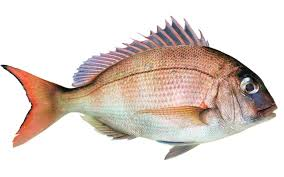
\includegraphics[width=3.125in,height=\textheight,keepaspectratio]{figuras/images.jpg}\end{minipage}%
\newline
\begin{minipage}{\linewidth}
Fonte: Google imagens\end{minipage}%

\end{figure}%

\subsection{Tabelas}\label{tabelas}

Tabelas são usadas para mostrar dados tabulares. Um exemplo de tabela é
a Tab.~\ref{tbl-1} abaixo.

\begin{longtable}[]{@{}lll@{}}
\caption{Exemplo de tabela: dados de
pessoas}\label{tbl-1}\tabularnewline
\toprule\noalign{}
Nome & Idade & Sexo \\
\midrule\noalign{}
\endfirsthead
\toprule\noalign{}
Nome & Idade & Sexo \\
\midrule\noalign{}
\endhead
\bottomrule\noalign{}
\endlastfoot
João & 20 & M \\
Maria & 25 & F \\
\end{longtable}

\subsection{Equações}\label{equauxe7uxf5es}

Black-Scholes (Equation~\ref{eq-black-scholes}) é um modelo matemático
que busca explicar o comportamento dos derivativos financeiros, mais
comumente opções:

\begin{equation}\phantomsection\label{eq-black-scholes}{
\frac{\partial \mathrm C}{ \partial \mathrm t } + \frac{1}{2}\sigma^{2} \mathrm S^{2}
\frac{\partial^{2} \mathrm C}{\partial \mathrm C^2}
  + \mathrm r \mathrm S \frac{\partial \mathrm C}{\partial \mathrm S}\ =
  \mathrm r \mathrm C 
}\end{equation}

\subsection{Código em Julia}\label{cuxf3digo-em-julia}

A seguir um código em Julia:

\vspace{0cm}

\begin{codelisting}

\caption{\label{lst-1}Customers Query}

\centering{

\begin{Shaded}
\begin{Highlighting}[]
\NormalTok{x }\OperatorTok{=} \FloatTok{1} \OperatorTok{+} \FloatTok{1}
\end{Highlighting}
\end{Shaded}

}

\end{codelisting}%

Este foi um exemplos do suporte a figuras, tabelas, equações e código em
Julia. Para mais informações sobre o suporte a figuras, tabelas,
equações e código (Cód.~\ref{lst-1}) em Julia, consulte
\url{https://quarto.org}.

\begin{codelisting}

\caption{\label{lst-2}Exemplo de código em Julia}

\centering{

\begin{Shaded}
\begin{Highlighting}[]
\NormalTok{x }\OperatorTok{=} \FloatTok{1} \OperatorTok{+} \FloatTok{1}
\end{Highlighting}
\end{Shaded}

}

\end{codelisting}%

É possível executar código em Julia/Python/R diretamente no Quarto.org.
O código é executado e o resultado é incluído no documento final.

\begin{Shaded}
\begin{Highlighting}[]
\NormalTok{m }\OperatorTok{=} \FloatTok{100} \CommentTok{\# kg}
\NormalTok{c }\OperatorTok{=} \FloatTok{3e8} \CommentTok{\# m/s}
\NormalTok{E }\OperatorTok{=}\NormalTok{ m }\OperatorTok{*}\NormalTok{ c}\OperatorTok{\^{}}\FloatTok{2} \CommentTok{\# J}

\FunctionTok{println}\NormalTok{(}\StringTok{"A energia é: "}\NormalTok{, E, }\StringTok{" Joules"}\NormalTok{)}
\end{Highlighting}
\end{Shaded}

\begin{verbatim}
A energia é: 9.0e18 Joules
\end{verbatim}

\begin{verbatim}
A energia é: 9.00e+18 Joules.
\end{verbatim}

Este foi um exemplos do suporte a figuras, tabelas, equações e código em
Julia (Cód.~\ref{lst-2}).

\subsection{Citando referências}\label{citando-referuxeancias}

A seguir um exemplo de citação de referências:

A citação de referências é feita como segue: GROTE; ANTONSSON
(\citeproc{ref-grote2009springer}{2009}).

\subsubsection{Fisheries and
Biodiversity}\label{fisheries-and-biodiversity}

Global freshwater resources include a diverse fish fauna comprising
close to 16,000 species (i.e.\textasciitilde47\% of all fishes
and\textasciitilde25\% of all vertebrates), with around 250 new species
described each year (\citeproc{ref-arthington2016fish}{ARTHINGTON et
al., 2016}; \citeproc{ref-eschmeyer2017catalog}{ESCHMEYER; FRICKE; LAAN,
2017}; \citeproc{ref-pelayo_villamil2015global}{PELAYO-VILLAMIL et al.,
2015}).

\chapter{Referencial Teórico}

\PROFESSOR{Apresentação teórica, baseada em referências bibliográficas, sobre o tema do trabalho.}

\section{Tema}\label{tema}

\section{Subtema}\label{subtema}

\subsection{Conceitos importantes}\label{conceitos-importantes}

\subsection{Etc}\label{etc}

\chapter{Metodologia}

\PROFESSOR{Descrição do que foi feito no trabalho.}

\chapter{Resultados e discussões}

\PROFESSOR{Resultados obtidos e o que eles significam.}

\chapter{Conclusão}

\PROFESSOR{Conclusões encontradas no trabalho}

\chapter{Trabalhos Futuros}

\chapter*{REFERÊNCIAS}

\phantomsection\label{refs}
\begin{CSLReferences}{0}{1}
\bibitem[\citeproctext]{ref-arthington2016fish}
ARTHINGTON, A. H. et al. Fish conservation in freshwater and marine
realms: status, threats and management. \textbf{Aquatic Conservation:
Marine and Freshwater Ecosystems}, v. 26, p. 838--857, 2016.

\bibitem[\citeproctext]{ref-eschmeyer2017catalog}
ESCHMEYER, W. N.; FRICKE, R.; LAAN, R. VAN DER. \textbf{Catalog of
Fishes, electronic version ({3 January 2017})}. San Francisco,
CACalifornia Academy of Sciences, 2017. Disponível em:
\textless{}\url{http://researcharchive.calacademy.org/research/ichthyology/catalog/fishcatmain.asp}\textgreater{}

\bibitem[\citeproctext]{ref-grote2009springer}
GROTE, K.-H.; ANTONSSON, E. K. \textbf{Springer handbook of mechanical
engineering}. {[}s.l.{]} Springer, 2009. v. 10

\bibitem[\citeproctext]{ref-pelayo_villamil2015global}
PELAYO-VILLAMIL, P. et al. Global diversity patterns of freshwater
fishes---potential victims of their own success. \textbf{Diversity and
Distributions}, v. 21, p. 345--356, 2015.

\end{CSLReferences}




\end{document}
